
\documentclass[10pt]{beamer}

\usepackage{graphicx}
\usepackage{xcolor}
\usepackage{amsfonts}
\usepackage{amsmath}
\usepackage{amssymb}
\usepackage[skip=10pt plus1pt] {parskip}

%Information to be included in the title page:
\title{Functions and Operations}
\author{UChicago Political Science Math Camp}
\institute{Ryan Gibbons \& Luke Cain}
\date{2025}

\begin{document}

\frame{\titlepage}

\begin{frame}
\frametitle{Today's Challenge}
\begin{itemize}
    \item You likely already know what a function is, or at least how to use one.
    \item We are going to \textit{formally redefine} what a function is and how we might expect to see them.
    \item Focus is not just on the outcome, but on the \textbf{process} and \textbf{definitions}.
\end{itemize}
\end{frame}

\begin{frame}{What you've seen already}
    You've likely seen a function expressed as $y$ or $f(x)$, like

    \[y = mx+b \quad \quad \quad f(x) = ax^2 + bx + c\]

    You also likely understand a graphed function, like

    \begin{center}
        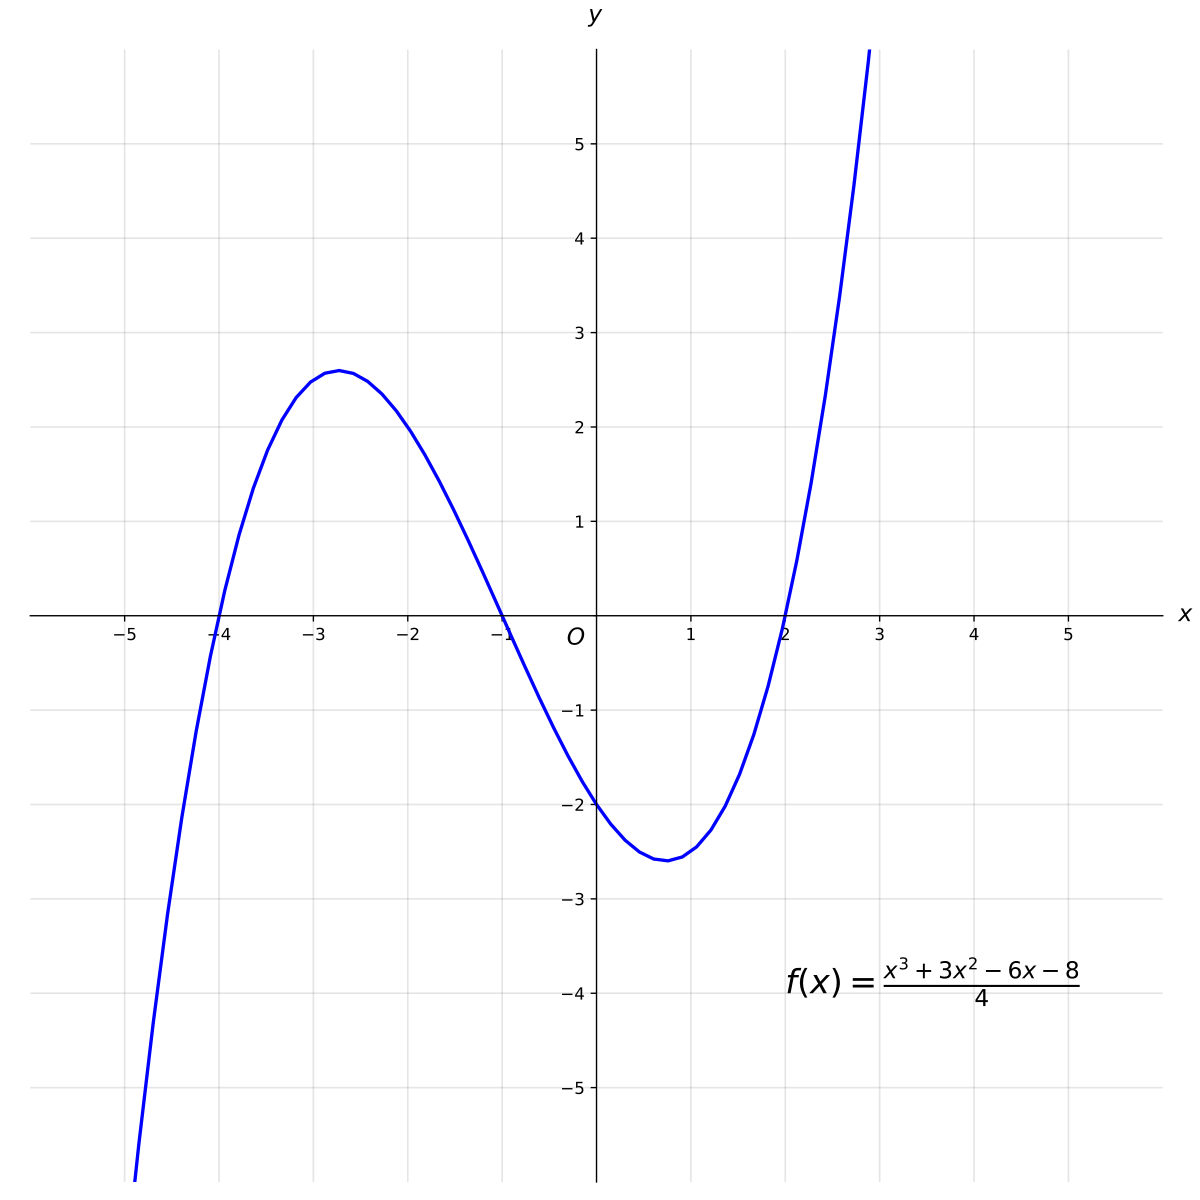
\includegraphics[width=4cm]{graphfunction.png}
    \end{center}
\end{frame}


\begin{frame}{What is a function?}

A function is a \textbf{mapping} of elements in some set (the \textbf{domain}) to elements in another set (the \textbf{codomain}):

\[f: A \rightarrow  B\]

Such that

\begin{itemize}
    \item $f$ labels the function
    \item $A$ is the domain (a set)
    \item $B$ is the codomain (also a set)
    \item $f(x\in A) \rightarrow f(x) \in B$
\end{itemize}
\pause
\textcolor{red}{A function is a rule transforming \textbf{inputs} into \textbf{outputs}.}
\end{frame}

\begin{frame}
    Let's start with an arbitrary function:

    \[A = \{51, 52,53,54,55\}\]

    \[B = \{\text{Dorchester, Kenwood, Kimbark, Woodlawn, University}\}\]

    Some function $g: A \rightarrow B$ could lend:

    \[g(51) = \text{Dorchester}\]
    \[g(52) = \text{Kimbark  }\]
    \[g(53) = \text{Woodlawn}\]
    \[g(54)=\text{University}\]
    \[g(55) = \text{Kenwood}\]

    Why? Because we said so!
\end{frame}

\begin{frame}{Functions in Political Science}
    We usually use a function to take some \textbf{variable}(s) as an input and return some \textbf{value} as an output. \\
\vspace{.5cm}
    \begin{itemize}
        \item A \textit{variable} is a symbol/letter that represents some unknown value
    \end{itemize}

    \vspace{.5cm}

    For example, we might take:

    \[Wealth: \{\text{Resources, Institutions, FDI, IR}\} \rightarrow GDP\]

    What might these parent sets look like? \\
    \pause
    \vspace{.5cm}
    What other functions in political science might we create?
\end{frame}

\begin{frame}{A Specific Social Science Function}
    How can we calculate GDP per capita from known, well-defined inputs? \\
    \vspace{.5cm}

    \begin{itemize}
        \item Through function notation $f: A \rightarrow B$
        \item Through some mathematical rule defining $f$ and returning $f(A) \in B$
    \end{itemize}
\end{frame}

\begin{frame}

In reality, we usually (but not always) work with more interpretable functions. Let us define:

\[C = \{x\in \mathbb{N}: x < 5\} \quad \quad \quad D = \{2 \cdot x \in \mathbb{N}:x < 5\}\]

Let us construct some function $h: C \rightarrow D$ such that $h(c) = 2c$:

\[C = \begin{Bmatrix}
    1 \\
    2 \\
    3 \\
    4 \\
   
\end{Bmatrix} \rightarrow h(c) = 2 c \rightarrow 
\begin{Bmatrix}
    h(1) = 2 \\
    h(2) = 4 \\
    h(3) = 6 \\
    h(4) = 8 \\
    
\end{Bmatrix} = D\]

So, $h$ is a very clean mapping from $C$ to $D$. But, this is a very limiting set of assumptions.

    
\end{frame}

\begin{frame}{What if we're not so lucky?}

Most often, we are using functions to map onto some real space $\mathbb{R}^n$. Let's redefine:

\[h: C \rightarrow \mathbb{R}\]

\[C = \begin{Bmatrix}
    1 \\
    2 \\
    3 \\
    4 \\
   
\end{Bmatrix} \rightarrow h(c) = 2 c \rightarrow 
\begin{Bmatrix}
    h(1) = 2 \\
    h(2) = 4 \\
    h(3) = 6 \\
    h(4) = 8 \\
    
\end{Bmatrix} \in \mathbb{R}\]

Now, we can broaden our codomain while preserving the nature of the function. But, there is a problem with this...

\end{frame}

\begin{frame}{Bijection}
A function is \textbf{bijective} iff it is both \textbf{injective} and \textbf{surjective}:

\begin{itemize}
    \item A function $f: A \rightarrow B$ is \underline{injective} iff $f$ maps every element in $A$ onto one and ONLY one element in $B$. (No two inputs return the same output.) \pause
    \item A function $f: A \rightarrow B$ is \underline{surjective} iff every element in $B$ is mapped by $f$ from an element in $A$.

\end{itemize}

Which condition(s) does $h: C \rightarrow \mathbb{R}$ not satisfy?
\end{frame}

\begin{frame}{Your Turn}

Explain whether or not the following functions are bijective, and why:

\begin{itemize}
    \item $f: \text{English letters} \rightarrow \{x \in \mathbb{N}: x \leq 26\}$

    Where $f$ returns for each letter its alphabetical order

    \item $g: \text{Animals in the zoo} \rightarrow \mathbb{R}_+$

    where $g$ returns for each animal its number of legs

    \item $h: \mathbb{Q}_+ \rightarrow \mathbb{R}_+$

    where $h$ returns a given arithmetic operation to its input
\end{itemize}

\end{frame}

\begin{frame}{Inverse Functions}

\begin{itemize}
        \item A function's inverse returns its domain element (input) given its codomain element (output).

        \item We express an inverse domain as $f^{-1}$, such that:

        \[f^{-1}:B \rightarrow A\]

        \[h(2) = 4 \quad \Rightarrow  \quad h^{-1}(4)=2\]

        \item This is useful for when we know what output we have (or want), but want to find an input to produce it. \\

        \vspace{.5cm}

        \textcolor{red}{How do we invert a non-bijective function?}
\end{itemize}

\end{frame}

\begin{frame}{An Oasis}

\begin{itemize}
    \item This is a formally rigorous way to define \textit{what you already know to be functions}: most ``functions" in algebra and calculus just map $\mathbb{R} \rightarrow \mathbb{R}$

    \item Take $f(x) = x^2$:

    \begin{itemize}
        \item It is implied that $x \in \mathbb{R}$, and we can see that $x \in \mathbb{R} \Rightarrow x^2 \in \mathbb{R}$ \pause
        \item The function takes every input $x$ and returns $x \times x$ \pause
        \item \textcolor{red}{Therefore, we have an input, an output, and a rule -- all well-behaved.}
        \pause
        \item ... right, guys?
    \end{itemize}
\end{itemize}


\end{frame}


\begin{frame}{Turns out $y=x^2$ is bullshit}
    \begin{itemize}
        \item The function as defined is \textbf{not injective}: $x,-x$ take on the same value of $f(x)$. \pause
        \item The function as defined is \textbf{not surjective}: it is not true that for every output $x \in \mathbb{R}$, we can recover $f^{-1}(x) \in \mathbb{R}$.
        \begin{itemize}
            \item We accommodate for this by implicitly assuming that $f(x) : \mathbb{R} \rightarrow \mathbb{R}_+$, but not rigorous if not specified...
        \end{itemize}
    \end{itemize}

We don't need bijection to work with functions, but it can be quite useful in modeling and proofs, and in considering probablistic distributions.
\end{frame}

\begin{frame}{Dealing with $y=x^2$ anyways}

\begin{itemize}
    \item Suppose we are working with $f(x) = x^2$, and ignore the ``bullshit" part
    \item Let's choose a few inputs; call that set $X$

\[X = \begin{Bmatrix}
    1 \\
    2 \\
    3 \\
    4 \\
   
\end{Bmatrix} \rightarrow f(x\in X) = x^2 \rightarrow 
\begin{Bmatrix}
    f(1) = 1 \\
    f(2) = 4 \\
    f(3) = 9 \\
    f(4) = 16 \\
    
\end{Bmatrix} \in \mathbb{R}\]
\item Now, let's plot these results.
\item What happens as $X$ begins to resemble $\mathbb{Q}$? What about $\mathbb{R}$?
\end{itemize}

\end{frame}

\begin{frame}{Desmos}
    A useful tool for visualizing functions\\

    \vspace{3cm}

    \begin{footnotesize}
        \textit{This is also a reminder for me to open it now}
    \end{footnotesize}
\end{frame}

\begin{frame}{Common Functions: Linear}

\begin{itemize}
    \item A constant relationship between $x$ and $f(x)$. Often expressed as 

    \[f(x) = mx + b\]

    where $m$ is the rate of change of $f(x)$ over a unit in $x$, and $b = f(0)$. \pause

    \item Or, if you're feeling adventurous,

    \[\exists \;a \in \mathbb{R} \; \;s.t.\; \;\frac{f(x_{i}) - f(x_{i-1})}{x_i - x_{i-1}} = a \;\;\forall \;i \in \mathbb{Z}\]
\end{itemize}

\end{frame}

\begin{frame}{Creating Linear Functions}

Assuming we haven't been given $m$ and $b$, we then:

\begin{itemize}
    \item Calculate $b = f(0)$ and

    \[m = \frac{\Delta f(x)}{\Delta x}\]

    Then plug in for $f(x) = mx+b$

    \item Or, for some given $m$ and pair $x,f(x) = (x_i, f(x_i))$, use \textbf{point-slope form}:

    \[m(x-x_i) = f(x) - f(x_i) \]

\end{itemize}

\end{frame}


\begin{frame}{Common Functions: Polynomial}

\begin{itemize}
    \item An algebraic function where inputs are multiplied by themselves some whole number of times over

    \item The highest exponent determines the \textbf{order} of the polynomial

    \item For example, a quadratic function might look like this:

    \[f(x) = ax^2 + bx + c\]

    and is a \textbf{second order polynomial}.

\end{itemize}

\end{frame}

\begin{frame}{Roots \& Wrangling Polynomials}

There's no uniform way to deal with polynomials, but there are a few common traits:

\begin{itemize}
    \item We often want to solve a polynomial for $f(x) = 0$. We call the $x$ value(s) that produce $f(x) = 0$ the \textbf{root(s)}.
    \begin{itemize}
        \item (Even if we want to solve $f(x) = a$, we will usually express $f(x) - a = 0$ and absorb $-a$ into $f(x)$.)
    \end{itemize} \pause
    \item The \textbf{most} roots a polynomial can have is equivalent to its order.
    \item We include $\sqrt{}$ functions as polynomials, where:

    \[x^\frac{a}{b} = \sqrt[b]{x^a}\]
\end{itemize}

\end{frame}


\begin{frame}{Common Functions: Exponential}

\begin{itemize}
    \item An exponential function consists of some constant being multiplied by itself a number of times dependent on $x$:

    \[f(x) = a^x\]

    \item A special case of the exponential function is when $a = e$, such that

    \[f(x) = e^x\]

    Which is sometimes abbreviated as

    \[f(x) = \exp({x})\]

\end{itemize}

\end{frame}

\begin{frame}{Wrangling Exponentials}

\begin{itemize}
    \item Exponential functions are \textbf{monotone}: they are either always increasing, or always decreasing (or never) \pause
    \item Although any $x \in \mathbb{Z}$ will return a real value for $f(a < 0) = a^x$, non-integer $x$'s do not return a real value for a negative $a$.
    \begin{itemize}
        \item Any non-integer $x$'s then call for a root of a negative number, which is only real for odd integers (contradiction)
    \end{itemize} \pause
    \item Many (most?) common asymmetric probability distributions are exponential (i.e., low values happen quite frequently while high values happen infrequently)
\end{itemize}

\end{frame}

\begin{frame}{Factorials!}
    Factorials are a very special family of functions with the following property:

    \[n! = 1 \times 2 \times 3 \times ... \times (n-1) \times n\]

    Note that factorials are discrete, and then only well-defined for $n \in \mathbb{N}$. The $\Gamma$ function allows us to represent factorials for $x \in \mathbb{R}, x \notin \mathbb{N}$. \\

    \vspace{.5cm}

    \textcolor{red}{We define $0! = 1$.}
\end{frame}

\begin{frame}{Wrangling Factorials}
    Factorials are rapidly-increasing, and only interpretable for small $n$ inputs (i.e. $10! = 3,628,800$). But, we often use some nifty division:

    \[\frac{(n+1)!}{n!} = \frac{1 \times 2 \times ... \times (n-1) \times n \times (n+1)}{1 \times 2 \times... \times (n-1) \times n}\]

    We can't easily calculate\footnote{by hand -- computers can go a bit higher, Google goes up to $170! = 7.25 \times 10^{306}$} $15!$ or $13!$, but it's very easy to calculate $\frac{15!}{13!}$ \\

    \vspace{.5cm}
\pause
    \textit{\textcolor{red}{The goal with factorials is to obtain a quotient!}}
\end{frame}

\begin{frame}{Logarithms}
\begin{itemize}
    \item Logarithms are the inverse of exponential functions, and help identify what exponent an input must be raised to in order to produce a given output

    \[x = b^y \quad \Rightarrow \quad \log_bx = y\]

    \item Though often not intuitive in calculation, can be very useful in regressing percentages or representing widely-distributed data

    \item (Formal theorists also like logarithms as they are monotonic and bijective W.R.T. the positive reals.)

    \item \textcolor{red}{Temperature vs. Decibels}
    
\end{itemize}
\end{frame}

\begin{frame}{Wrangling Logarithms}
    \begin{itemize}
   \item You may be used to assuming $b = 10$ if unspecified, such that

    \[\log 100 = 2\]

    This is commonly used for data analytics and empirical measures.

    \item But, in advanced mathematics (and formal theory), we sometimes assume that $b = e$, represented as

    \[\ln x = n \quad \Rightarrow \quad e^x = n\]

    \textit{sometimes even if written as $\log$ and not as $\ln$.}
    \end{itemize}
\end{frame}

\begin{frame}{Multivariable Functions}
\begin{itemize}
    \item It's not all that often that we're only working with a single input and output. For example, projected GDP is a function of both growth rate and present GDP.

    \item We can represent a multivariable function as:

    \[f(x,y), \; f(x,y,z), \; f(w,x,y,z),...\]

    Where $f$ returns a single output given each of these inputs. \pause

    \item Informally, we can think of the output of $f(x)$ as a line, and $f(x,y)$ as a surface, but difficult to conceptualize beyond that
    \item We will learn how to wrangle these in the calculus unit (it's easier than it sounds)
\end{itemize}
\end{frame}

\begin{frame}{Mapping Between Different Dimensions}
\begin{itemize}
    \item Recall that our ``conventional" single-variable function maps $f: \mathbb{R} \rightarrow \mathbb{R}$
    \item When we have multiple variables, though, we are mapping from a ``space" of those variables. So, it might be the case that for $f(x,y)$,

    \[f: \mathbb{R}^2 \rightarrow \mathbb{R}\]

    \[f^{-1}: \mathbb{R} \rightarrow \mathbb{R}^2\]

    \item This can be much harder, though... to apply an inverse function, we often want only one space

\end{itemize}
\end{frame}

\begin{frame}{Hints for Multivariable Functions}
\begin{itemize}
    \item Hint \#1: use $\mathbb{R}^n$ for $n$ input variables \pause
    \item Hint \#2: we are often just mapping something onto $\mathbb{R}$, which means that for the input(s), \textit{we just recover a single numeric output.} \pause
    \item Hint \#3: don't try to visualize functions involving beyond $\mathbb{R}^3$ (and really not beyond $\mathbb{R}^2$)
\end{itemize}
\end{frame}


\begin{frame}{A Few Helpful Notes}
\begin{itemize}
    \item The \textbf{support} of a function is the set of reals which returns a non-zero output
    \item It is almost always helpful to use \textbf{Desmos} to plot a function that you cannot visualize
    \item Functions can be ``summed": it can be the case that one term of $f$ is polynomial and another term is exponential, etc.
\end{itemize}
    
\end{frame}


\begin{frame}{Taking A Sum}
    \begin{itemize}
        \item We often want to calculate the total amount of individual values:
        \begin{itemize}
            \item Total wealth is the sum of individual wealth for every member of the population
            \item Global emissions are the sum of national emissions for every nation in the world
            \item Total contributions is the sum of all individual contributions for every contributor
        \end{itemize}
        \item Or, even if not substantively, we just want to use simpler notation
    \end{itemize}
\end{frame}

\begin{frame}{Summation Operation}
    To take a sum, we use the summation operation:

    \[X = \sum_{i=a}^{b} x_i\]

    Where

    \begin{itemize}
        \item $X$ is the total sum
        \item $i$ is the \textbf{index} (indexes \underline{must} be natural numbers)
        \item $a$ is the \textbf{lower bound}
        \item $b$ is the \textbf{upper bound}
    \end{itemize}
\end{frame}

\begin{frame}{Some Examples}

We can express $1+2$ as

\[\sum_{i=1}^2 i = 3 \]

And even use set-builder notation

\[\sum_{i=1}^2 x_i: x \in \mathbb{N} = 3\]

We can get more complicated, but the concept stays the same:

\[f(x) = \sum_{i = 1}^N \frac{\lambda}{\sqrt{i}}\; = \;\frac{\lambda}{\sqrt{1}} \;+ \;\frac{\lambda}{\sqrt{2}}\; +\; ... \;+ \;\frac{\lambda}{\sqrt{N-1}} \;+ \;\frac{\lambda}{N}\]

\end{frame}

\begin{frame}{More Summation}
\begin{itemize}
    \item Sometimes our domain may even be the bounds:

    \[f(x) = \sum_{i=1}^x \frac{1}{2^i}\]

    \item But, note that we must specify where we are starting from (often, but not always, either $i = 0$ or $i = 1$)
    \item Any symbol can be used as an index, but we most often use either $i,k,n$
\end{itemize}
\end{frame}

\begin{frame}{Wrangling Summations}
\begin{itemize}
    \item A summation expression acts like a distributive term, and can be treated as such:

    \[\sum_{i=1}^{N}  a \cdot f(i) = a \cdot \sum_{i=1}^{N}f(i)\]

    but

    \[\sum_{i=1}^{N} (f(i))^b \neq  \Big( \sum_{i=1}^N f(i) \Big)^b\]
\end{itemize}
\end{frame}

\begin{frame}{Products}
    A nearly-identical process can be used to multiply, rather than add, a series of indexed values:

        \[X = \prod_{i=a}^{b} x_i\]

    Where

    \begin{itemize}
        \item $X$ is the total product
        \item $i$ is the \textbf{index} (indexes \underline{must} be natural numbers)
        \item $a$ is the \textbf{lower bound}
        \item $b$ is the \textbf{upper bound}
    \end{itemize}
\end{frame}

\begin{frame}{Sequences}
    Sequences are special cases of functions:
    
    \begin{itemize}
        \item A \textbf{sequence} is a function $a: \mathbb{N} \rightarrow \mathbb{R}$
    \end{itemize}

    Specifically, sequences have \textit{discrete inputs} and \textit{indexed outputs}
\end{frame}

\begin{frame}{Series}
Series are sums of infinitely many numbers:

\[\sum_{k=1}^\infty \frac{1}{2^k}\]

\[\Rightarrow = \frac{1}{2} + \frac{1}{4} + \frac{1}{8} + ...\]

How might we define a series in relation to a sequence?
\end{frame}

\begin{frame}{A Very Important Series}
\[\sum_{k=0}^\infty \frac{1}{n!}= e\]    
\end{frame}



\end{document}